% !TEX encoding = UTF-8
% !TEX TS-program = pdflatex
% !TEX root = ../tesi.tex

%**************************************************************
\chapter{Serie A 2021/2022 dataset }
\label{cap:dataset}
%**************************************************************

\intro{Nel seguente capitolo verrà descritta la raccolta dati effettuata per costruire il \emph{dataset} riguardante le partite di calcio della Serie A italiana della stagione 2021/2022 e la struttura di tale \emph{dataset}.}\\

%**************************************************************
\section{Serie A 2021/2022}

L'analisi effettuata ha preso in considerazione le partite della Serie A italiana della stagione 2021/2022. La Serie A è un torneo che comprende 20 squadre sparse per tutta l'Italia, alcune anche della stessa città, come ad esempio Milan e Inter per Milano. \\
Tale torneo è organizzato con una struttura \emph{Double-Round-Robin}, dove ogni squadra affronta due volte le altre 19 avversarie del torneo. Vi è quindi una partita di andata e una di ritorno. In base al sorteggio necessario alla creazione del calendario delle partite si decide quale delle due partite sarà giocata in casa oppure fuori casa (in casa dell'avversario). \\
Il torneo della stagione 2021/2022 è iniziato il 22 Agosto con Inter - Genoa e si è concluso il 22 Maggio con le partite Salernitana - Udinese e Venezia - Cagliari, per un totale 380 partite giocate, suddivise in 38 turni, ciascuno composto da 10 partite.

\subsection{Ranking}
Le squadre di calcio sono classificate in base all'ordine dei punti che hanno totalizzato al termine della stagione. In un torneo calcistico, per ogni partita, la squadra vincitrice guadagna tre punti, la squadra sconfitta guadagna nessun punto, mentre, in caso di pareggio, entrambe le squadre guadagnano un punto. Nel torneo della Serie A chi guadagna più punti vince il campionato, mentre chi si classifica tra le ultime tre retrocede alla lega inferiore, la Serie B. Il posto delle tre squadre retrocesse verrà preso da tre squadre della Serie B che hanno guadagnato la promozione alla Serie A.\\ 
La classifica della stagione 2021/2022 è riportata nella Figura \ref{fig:ranking}.

\begin{figure}[h]
	\begin{center}
		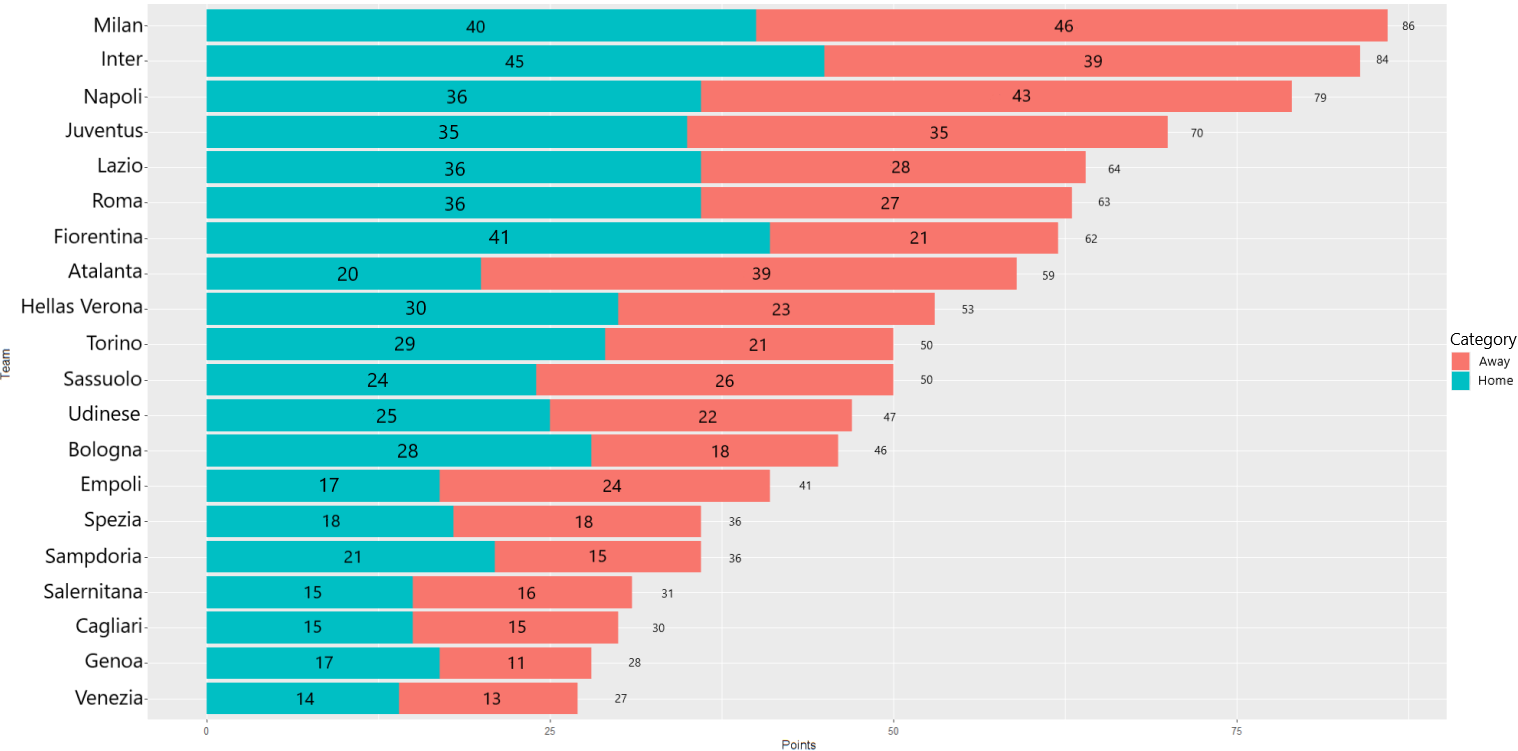
\includegraphics[height = 10cm, width = 14cm]{ranking.png}
		\caption{Grafico della classifica del campionato italiano della Serie A 2021/2022. Le barre di color azzurro indicano i punti che la squadra ha guadagnato in partite casalinghe. Le barre di color rosa indicano i punti che la squadra ha guadagnato in partite fuori casa.
		} 
		\label{fig:ranking}
	\end{center}
\end{figure}
\begin{comment}[!htb]%
	
	\renewcommand{\arraystretch}{1.7}
	\centering
	\begin{tabular}{c c c c}
		\hline	
		
		\textbf{Posizione} & \textbf{Squadra} & \textbf{Punti} & \textbf{ \% punti in casa}  \\	
		\hline			
		1 & Milan & 86 & 0.47\\
		2 & Inter & 84 & 0.54\\
		3 & Napoli & 79 & 0.46\\
		4 & Juventus & 70 & 0.50\\
		5 & Lazio & 64 & 0.56\\
		6 & Roma & 63 & 0.57\\
		7 & Fiorentina & 62 & 0.66\\
		8 & Atalanta & 59 & 0.33\\
		9 & Hellas Verona & 53 & 0.57\\
		10 & Torino & 50 & 0.58\\
		11 & Sassuolo & 50 & 0.48\\
		12 & Udinese & 47 & 0.53\\
		13 & Bologna & 46 & 0.61\\
		14 & Empoli & 41 & 0.42\\
		15 & Sampdoria & 36 & 0.58\\
		16 & Spezia & 36 & 0.50\\
		17 & Salernitana & 31 & 0.48\\
		18 & Genoa & 30 & 0.50\\
		19 & Cagliari & 28 & 0.61\\
		20 & Venezia & 27 & 0.52\\
		\hline
		& & & \\
		
	\end{tabular} \hbox{}
	
	\caption{La tabella mostra i punti guadagnati da ogni squadra con il loro piazzamento. Inoltre viene mostrata la percentuale di punti guadagnati in casa.} \label{tab:ranking}
\end{comment}

%**************************************************************
\section{Costruzione del dataset}

Al giorno d'oggi, nelle partite di calcio professionistico viene raccolta un'enorme quantità di variabili. Ad esempio, per ogni squadra è noto il tempo in percentuale del possesso della palla e il numero di tiri in porta in una determinata partita. L'obbiettivo principale di questo lavoro è determinare l'influenza che queste variabili hanno sull'esito della partita. \\
A tale scopo, sono state raccolte un gran numero di variabili che si suppone essere associate all'esito della partita.\\
Tali dati sono stati offerti dal sito web \textit{\cite{fbref}}, un sito web dedicato al tracciamento delle statistiche relative ai calciatori e alle squadre di calcio di tutto il mondo. \\
Il sito web \textit{\cite{fbref}} mette a disposizione i dati sotto forma di tabelle che possono essere modificate per mantenere solo i dati di nostro interesse.\\
\begin{figure}[!htb]
	\begin{center}
		
\includegraphics[scale=0.30]{logo.png}
		\caption{Logo di FBref.} 
		Source: \url{https://fbref.com}
		\label{fig:logo}
	\end{center}
\end{figure}
Dunque, per ogni squadra che ha partecipato alla stagione 2021/2022 di Serie A, sono state esportate le variabili di interesse per ogni partita giocata, selezionando le macro-aree opportune e adattando le tabelle per ottenere solo i dati utili. Le varie tabelle hanno composto un file Excel divenuto il \emph{dataset} per le analisi svolte nelle tesi.

\section{Struttura del dataset}
Il \emph{dataset} risultante dalla raccolta dati è composto da 760 righe e 35 colonne. Ogni riga riguarda una specifica partita di calcio giocata dalla squadra indicata nella colonna \textsf{Team} contro la squadra indicata nella colonna \textsf{Vs}. Ogni riga contiene informazioni riguardati solo la squadra indicata in \textsf{Team} fatta eccezione per la data della partita (\textsf{Date}), il turno (\textsf{Round}) e gli spettatori (\textsf{Spec}). Quindi, per ogni partita esistono due righe, una per ciascuna squadra coinvolta. Come risultato finale, ogni squadra appare nella colonna \textsf{Team} 38 volte e, siccome il numero totale di squadre è 20, si ottengono 760 righe. %Per quanto riguarda le colonne se ne discuterà nella prossima sottosezione. \\
La Tabella \ref{tab:db} mostra un breve estratto dei dati riguardanti le prime tre partite della stagione. 
\begin{table}[!ht]%
	
	\renewcommand{\arraystretch}{1.7}
	\centering
	\begin{tabular}{c c c c c c c c c  }
		\hline	
		
		\textbf{Date} & \textbf{AtHome} & \textbf{Res} & \textbf{GF} & \textbf{GA} & \textbf{Team} & \textbf{Vs} & \textbf{Poss} & \textbf{...}   \\	
		\hline	
		21/08/2021 & TRUE & 1 & 4 & 0 & Inter & Genoa & 0,59 & ... \\
		... & ... & ... & ... & ... & ... & ... & ... & ... \\
		22/08/2021  & TRUE & 1 & 2 & 0 & Napoli & Venezia & 0,56 & ... \\
		... & ... & ... & ... & ... & ... & ... & ... & ...  \\
		23/08/2021  & FALSE & 1 & 1 & 0 & Milan & Sampdoria & 0,51 & ... \\		
		... & ... & ... & ... & ... & ... & ... & ... & ... \\
		21/08/2021  & FALSE & -1 & 0 & 4 & Genoa & Inter & 0,41 & ... \\
		... & ... & ... & ... & ... & ... & ... & ... & ...  \\
		22/08/2021  & FALSE & -1 & 0 & 2 & Venezia & Napoli & 0,44 & ... \\
		... & ... & ... & ... & ... & ... & ... & ... & ...  \\
		23/08/2021 1 & TRUE & 1 & 0 & 1 & Sampdoria & Milan & 0,49 & ... \\
		... & ... & ... & ... & ... & ... & ... & ... & ...  \\
		\hline
		& & & & & & & & \\
		
		
		
	\end{tabular} \hbox{}
	
	\caption{La tabella mostra un estratto del \emph{dataset} utilizzato i cui dati sono stati ricavati da FBref.} \label{tab:db}
\end{table}

Come scritto precedentemente all'interno del \emph{dataset} sono presenti 35 colonne. Oltre alle già citate \textsf{Date}, \textsf{Round} e \textsf{Spec} che hanno solo un valore di completezza dei dati, le restanti 32 colonne sono le possibili variabili che possono influenzare l'esito della partita.
Le covariate sono state raggruppate nelle seguenti cinque macro-aree:
\begin{itemize}
	\item dati generali,
	\item dati relativi ai tiri,
	\item dati possesso,
	\item dati passaggi,
	\item dati difensivi,
\end{itemize}

che sono illustrate di seguito.
%\pagebreak

\subsection{Dati generali}
In questo gruppo sono presenti le variabili legate a statistiche che non fanno parte di una precisa macroarea ma che descrivono più genericamente la partita giocata. 

Le possibili covariate sono le seguenti:
\begin{itemize}
	\item \textsf{AtHome}: indica se la squadra specificata della variabile \textsf{Team} gioca nel proprio stadio, quindi in casa oppure fuori casa. Per indicare se la squadra gioca in casa viene messo come valore \texttt{TRUE} altrimenti \texttt{FALSE}. \\
	Come mostrato dalla Figura \ref{fig:ranking}, la quale indica quanti punti sono stati vinti in casa per ogni squadra, ci sono 11 squadre che hanno avuto un leggero vantaggio nel giocare in casa le partite di calcio rispetto a altre sei squadre che hanno avuto l'effetto opposto, mentre le rimanti tre hanno avuto un effetto nullo.\\
	\item \textsf{Res}: indica se la squadra specificata della variabile \textsf{Team} ha vinto, pareggiato o perso la partita. Per indicare se ha vinto viene inserito il valore 1, se ha pareggiato 0, altrimenti se ha perso -1. \textsf{Res} sarà la variabile risposta.
	\item \textsf{GF}: indica il numero di gol fatti dalla squadra specificata della variabile \textsf{Team}. \\
	È stata inserita perché può permettere di valutare la qualità della fase offensiva della squadra e quindi ci si aspetta che possa essere utile ai fini dell'analisi.
	\item \textsf{GA}: Indica il numero di gol subiti dalla squadra specificata della variabile \textsf{Team} e quindi fatti dalla squadra indicata nella variabile \textsf{Vs}. \\
	Essa può essere utile perché subire pochi gol incide positivamente sull'esito della partita, limitando l'esposizione della squadra ad uno sbilanciamento in attacco per recuperare lo svantaggio e quindi rischiando maggiormente di subire ulteriori gol dagli avversari. Inoltre, è un fatto riconosciuto che aver la miglior difesa del campionato è associato ad una maggiore probabilità di vittoria del campionato (vedi \textit{\cite{catenaccio}}).
	\item \textsf{Team}: indica il nome della squadra a cui i dati della riga fanno riferimento.
	\item \textsf{Vs}: indica il nome della squadra avversaria.
	
	\item \textsf{Fld}: indica il numero di falli fatti dai giocatori della squadra specificata della variabile \textsf{Team}. \\
	Questa variabile è stata inserita per capire se una squadra adotta un gioco più fisico/tattico. In questo caso sarà più propensa a interrompere il gioco della squadra avversaria e a commettere più falli. Si vuole perciò capire come questa variabile possa essere associata all'esito della partita, ricordando però che una squadra che commette molti falli è più soggetta a ricevere cartellini gialli o rossi che condizionano la prestazione dei giocatori.
	\item \textsf{Fls}: indica il numero di falli subiti dai giocatori della squadra specificata della variabile \textsf{Team} da parte della squadra avversaria specificata della variabile \textsf{Vs}. \\
	Si è deciso di inserire questa covariata perché un alto numero di falli può portare a molte interruzioni della manovra di gioco e quindi permettere alla squadra avversaria di riorganizzarsi.
	
	\item \textsf{Off}: indica il numero di volte che la squadra specificata della variabile \textsf{Team} è finita in fuorigioco. Un calciatore si trova in posizione di fuorigioco quando una qualsiasi parte del suo corpo, fatta eccezione per braccia e mani, si trova nella metà campo avversaria ed è più vicina alla linea di porta avversaria, sia rispetto al pallone che rispetto al penultimo giocatore difendente avversario, portiere compreso nel caso in cui un compagno di questi è più vicino alla linea di porta. Una rappresentazione grafica del fuorigioco è mostrata nella Figura \ref{fig:offside}.
	
	\begin{figure}[!ht]
		\begin{center}
			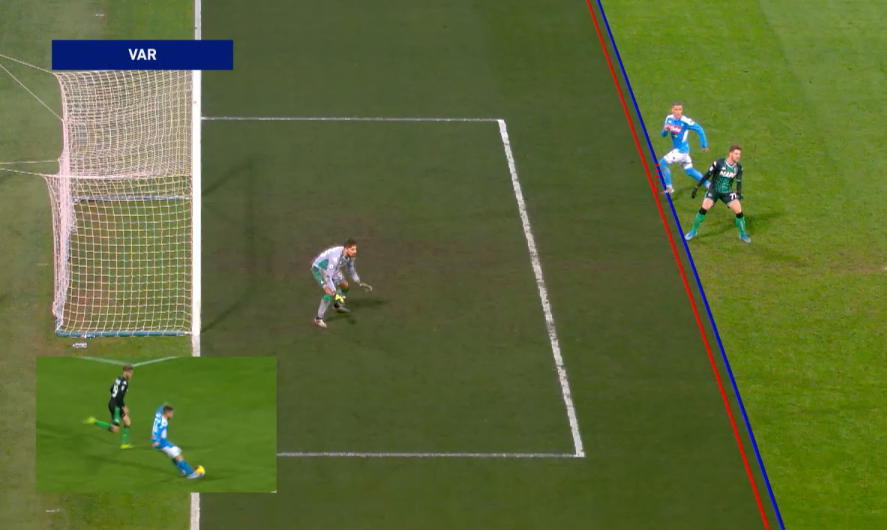
\includegraphics[scale=0.50]{var.png}
			
			\caption{Rappresentazione del fuorigioco} \label{fig:offside}
			Source: \url{https://sport.sky.it/calcio/2021/10/05/fifa-figc-var-fuorigioco}
		\end{center}
	\end{figure}
	
	Questa variabile è stata inserita perché, se una squadra viene colta molte volte in fuorigioco allora il suo gioco sarà interrotto generando un vantaggio alla squadra avversaria che farà ripartire la sua azione a proprio favore.
	
\end{itemize}

\subsection{Dati relativi ai tiri}

In questo gruppo sono presenti le variabili collegata alla fase offensiva della squadra in esame.

\begin{itemize}
	
	\item \textsf{Sh}: indica il numero di tiri totali fatti dalla squadra specificata della variabile \textsf{Team}. Quindi vengono conteggiati il numero di tiri in porta più i tiri fuori dalla porta. \\
	Una squadra che effettua tanti tiri ha più probabilità di segnare un gol. Occorre però capire quanto è precisa una squadra nel centrare la porta.
	\item \textsf{SoT}: Indica il numero di tiri in porta totali fatti dalla squadra specificata della variabile \textsf{Team}. \\
	Una squadra con un alto valore di tiri in porta è più probabile che possa segnare un gol. \texttt{SoT} permette di capire quanto è precisa in combinazione con \texttt{Sh} la squadra di calcio nel centrare la porta.
	\item \textsf{G/Sh}: indica la proporzione tra gol e tiri fatti dalla squadra specificata della variabile \textsf{Team}. \\
	Questo può permettere di capire quanto la produzione di tiri della squadra è efficace o meno. Con \texttt{Sh} e \texttt{SoT} si riesce a valutare quanto sia offensiva la squadra, cioè se essa gioca costantemente in attacco o utilizza la tattica "difesa e contropiede". Inoltre, permette di capire quanto la squadra sia precisa nell'effettuare i tiri in porta.
\end{itemize}

\subsection{Dati relati al possesso}

In questo gruppo sono contenute le variabili collegate al possesso della palla. 

\begin{itemize}
	
	\item \textsf{Poss}: indica la quantità di tempo (in percentuale) di possesso palla durante una partita di calcio per la squadra specificata della variabile \textsf{Team}. Nel gioco del calcio, con il termine “possesso palla” si intende un’azione manovrata di due o più giocatori che riescono a passarsi la palla evitando i contrasti degli avversari. Durante la partita, ogni volta che una squadra ha il dominio della palla si dice che questa squadra è in fase di “possesso palla”, quindi in questa variabile viene indicato quanto questa fase è durata nell'intera partita.\\
	Il metodo più comune utilizzato per calcolare il possesso palla di una squadra si basa sull'utilizzo di tre cronometri, uno per ciascuna formazione più uno per i tempi morti. Quando un giocatore della squadra A tocca un pallone che prima era in possesso della squadra B, il cronometro della squadra A parte e quello della squadra B si ferma e così via. Il terzo cronometro registra il tempo in tutte le situazioni di palla inattiva, ad esempio, rimesse laterali, calci di punizione ecc... I tempi vengono poi trasformati in percentuali. Per una registrazione più sofisticata, si possono utilizzare ventidue cronometri, uno per ogni giocatore.\\
	La variabile è stata inserita perché, la supremazia nel possesso palla è solitamente desiderabile e utile, dati i seguenti vantaggi:
	\begin{itemize}
		\item spingere l’avversario a muoversi verso la palla per allontanarlo dalla difesa della propria porta per poi sorprenderlo negli spazi lasciati incustoditi.   
		\item modulare il ritmo della gara, ad esempio, se una squadra sta vincendo con un gol di scarto, "congela" il risultato mantenendo il possesso della palla in modo da non ricevere attacchi da parte della squadra avversaria.
	\end{itemize}
	Il possesso palla però non garantisce la vittoria. Produrre un possesso palla "sterile", cioè senza che questo porti alla produzione di azioni offensive, può esporre la squadra in possesso della palla a contropiedi nel caso in cui la palla venga persa e quindi all'alto rischio di subire gol perché sbilanciata e non ben posizionata. Vedremo di seguito quali variabili possono essere utili per capire se il possesso palla fatto dalla squadra è "sterile" oppure no.
	
	\item \textsf{ToDefPen}: indica il numero di tocchi fatti dai giocatori della squadra specificata della variabile \textsf{Team} nella propria area di rigore. \\
	Questa variabile è stata inserita perché può essere utile per capire come venga gestito il possesso della palla. Se vi è un alto numero di tocchi, vuol dire che la squadra subisce molto la pressione della squadra avversaria, viceversa cerca di fare un gioco più offensivo. Questa variabile, in combinazione con le variabili \textsf{ToDef3rd}, \textsf{ToMid3rd}, \textsf{ToAtt3rd} e \textsf{ToAttPen} permette di capire se il possesso della palla fatto della squadra sia utile e porti benefici ai fini del risultato oppure sia sterile. Inoltre, si vuole capire in che misura come \textsf{ToDefPen} influenza il risultato della partita con un alto o un basso valore di numero di tocchi nella propria area di rigore, la cui area è indicata nella Figura \ref{fig:penalty}.
	
	\begin{figure}[!ht]
		\begin{center}
			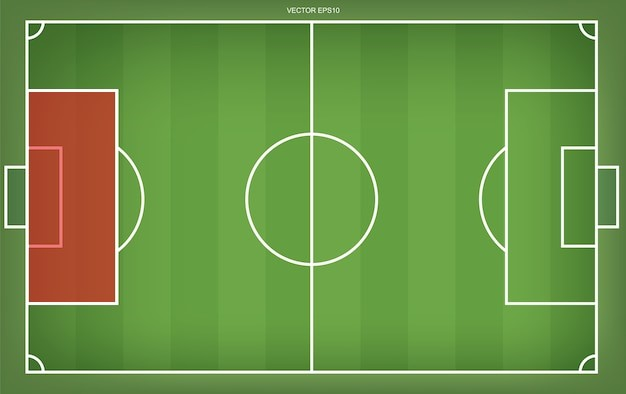
\includegraphics[scale=0.58]{rigore.jpg}
			\caption{In rosso l'area di rigore in un campo da calcio.}
			Source: \url{https://it.freepik.com/foto-vettori-gratuito/campo-da-calcio} 
			\label{fig:penalty}
		\end{center}
	\end{figure}
	
	
	\item \textsf{ToDef3rd}: indica il numero di tocchi fatti dai giocatori della squadra specificata della variabile \textsf{Team} nella propria mediana o trequarti difensiva. \\
	Questa variabile è stata inserita perché può essere utile per capire come venga gestito il possesso della palla. Se vi è un alto numero di tocchi, vuol dire che la squadra cerca di mantenere il possesso palla creando poche azioni offensive, viceversa cerca di fare un gioco più offensivo. Questa variabile, in combinazione con \textsf{ToDefPen}, \textsf{ToMid3rd}, \textsf{ToAtt3rd} e \textsf{ToAttPen}, permette di capire se il possesso della palla fatto della squadra sia utile e porti benefici ai fini del risultato oppure sia sterile. Inoltre, si vuole capire in che misura \textsf{ToDef3rd} influenza il risultato della partita con un alto o un basso valore di numero di tocchi nella propria mediana la cui area, è indicata nella Figura \ref{fig:def}.
	
	\begin{figure}[!ht]
		\begin{center}
			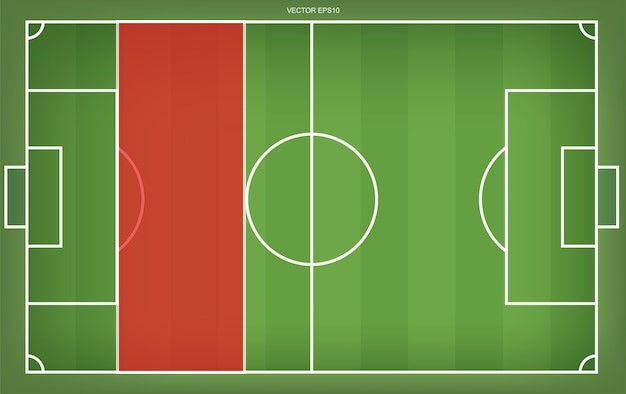
\includegraphics[scale=0.58]{mid.jpg}
			\caption{In rosso la mediana nel campo da calcio.} 
			Source: \url{https://it.freepik.com/foto-vettori-gratuito/campo-da-calcio} 
			\label{fig:def}
		\end{center}
	\end{figure}
	\item \textsf{ToMid3rd}: indica il numero di tocchi fatti dai giocatori della squadra specificata della variabile \textsf{Team} a centrocampo. \\
	Questa variabile è stata inserita perché può essere utile per capire come venga gestito il possesso della palla. Se vi è un alto numero di tocchi, vuol dire che la squadra cerca di mantenere il possesso palla cercando di creare delle azioni offensive, viceversa cerca di fare un gioco più difensivo. Questa variabile, in combinazione con le variabili \textsf{ToDefPen}, \textsf{ToDef3rd}, \textsf{ToAtt3rd} e \textsf{ToAttPen}, permette di capire se il possesso della palla fatto dalla squadra sia utile e porti benefici ai fini del risultato oppure sia sterile. Inoltre, si vuole capire in che misura \textsf{ToMid3rd} influenza il risultato della partita con un alto o un basso valore di numero di tocchi a centrocampo la cui area, è indicata nella Figura \ref{fig:cen}.
	
	\begin{figure}[!ht]
		\begin{center}
			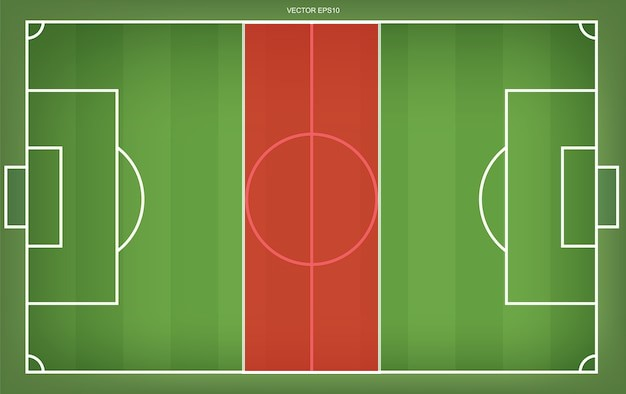
\includegraphics[scale=0.58]{cen.jpg}
			\caption{In rosso il centrocampo nel campo da calcio.}
			Source: \url{https://it.freepik.com/foto-vettori-gratuito/campo-da-calcio}  
			\label{fig:cen}
		\end{center}
	\end{figure}
	
	\item \textsf{ToAtt3rd}: indica il numero di tocchi fatti dai giocatori della squadra specificata della variabile \textsf{Team} nella trequarti dell'avversario. \\
	Questa variabile è stata inserita perché può essere utile per capire come venga gestito il possesso della palla. Se vi è un alto numero di tocchi, vuol dire che la squadra cerca di mantenere il possesso palla per effettuare una pressione sulla squadra avversaria affinché si possano creare degli spazi per delle azioni offensive, viceversa cerca di fare un gioco molto più difensivo. Questa variabile, in combinazione con le variabili \textsf{ToDefPen}, \textsf{ToDef3rd}, \textsf{ToMid3rd} e \textsf{ToAttPen}, permette di capire se il possesso della palla fatto della squadra sia utile e porti benefici ai fini del risultato oppure sia sterile. Inoltre, si vuole capire in che misura \textsf{ToAtt3rd} influenza il risultato della partita con un alto o un basso valore di numero di tocchi nella trequarti dell'avversario la cui area, è indicata nella Figura \ref{fig:treq}.
	
	\begin{figure}[!ht]
		\begin{center}
			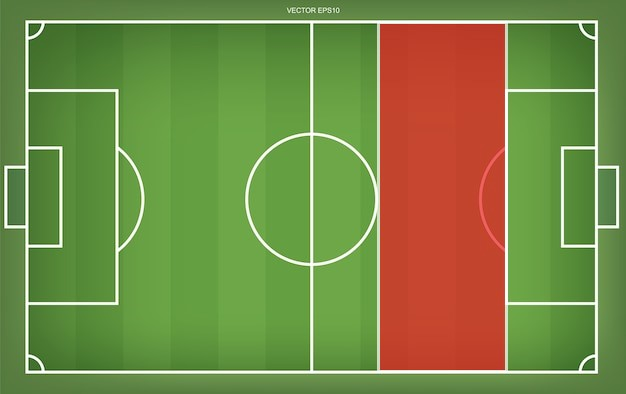
\includegraphics[scale=0.58]{treq.jpg}
			\caption{In rosso la trequarti dell'avversario nel campo da calcio.} 
			Source: \url{https://it.freepik.com/foto-vettori-gratuito/campo-da-calcio} 
			\label{fig:treq}
		\end{center}
	\end{figure}
	
	\item \textsf{ToAttPen}: indica il numero di tocchi fatti dai giocatori della squadra specificata della variabile \textsf{Team} a nell'area di rigore dell'avversario. \\
	Questa variabile è stata inserita perché può essere utile per capire come venga gestito il possesso della palla. Se vi è un alto numero di tocchi, vuol dire che la squadra cerca di mantenere il possesso palla applicando un'alta pressione sulla squadra avversaria affinché si possano creare molte occasioni da gol in area, viceversa o la squadra subisce troppo la pressione dell'avversario oppure tende ad avere un gioco molto difensivo. Questa variabile, in combinazione con le variabili \textsf{ToDefPen}, \textsf{ToDef3rd}, \textsf{ToMid3rd} e \textsf{ToAtt3rd} permette di capire se il possesso della palla fatto della squadra sia utile e porti benefici ai fini del risultato oppure sia sterile. Inoltre, si vuole capire in che misura \textsf{ToAttPen} influenza il risultato della partita con un alto o un basso valore di numero di tocchi nell'area di rigore dell'avversario.
	\item \textsf{ToDist}: Indica la distanza totale, espressa in metri, in cui un giocatore della squadra specificata della variabile \textsf{Team} si è mosso con la palla in qualsiasi direzione, controllandola con i piedi.\\
	Questa variabile è stata inserita perché permette di comprendere se il possesso della palla sia stato statico, ovvero i giocatori si sono mossi poco senza avanzare, oppure no. Sarà di interesse analizzare se un alto valore di metri percorsi con palla al piede possa essere utile ad ottenere la vittoria.
	
\end{itemize}

\subsection{Dati relativi ai passaggi}
%SCRIVI SOLO "INDICA" SU TUTTE LE PROSSIME COME HO FATTO PRIMA: Tale variabile indica => indica

In questo gruppo vi sono raggruppate le variabili collegate ai passaggi della palla.

\begin{itemize}
	
	
	\item \textsf{PAtt}: Indica il numero di tutti i passaggi tentati dai giocatori della squadra specificata della variabile \textsf{Team}. \\
	Utile a capire quanto la squadra sia incline a tentare i passaggi.
	
	\item\textsf{PCmp\%}: Indica la percentuale di passaggi riusciti ai giocatori della squadra specificata della variabile \textsf{Team}.\\ 
	È stata inserita perché permette di capire quanti passaggi siano andati a buon fine tra tutti quelli tentati e quindi ricavare la precisione dei giocatori della squadra.
	\item \textsf{SPAtt}: Indica il numero di passaggi corti tentati dai giocatori della squadra specificata della variabile \textsf{Team}. Per passaggi corti si intendono tutti quelli effettuati all'interno di una lunghezza tra i tre e quattordici metri.\\
	È stata inserita per capire se un alto numero di passaggi corti possa essere determinanti ai fini dell'esito della partita. 
	
	\item \textsf{SPCmp\%}: Indica la percentuale di passaggi corti riusciti ai giocatori della squadra specificata della variabile \textsf{Team}. \\
	È stata inserita perché permette di capire quanti passaggi andati a buon fine tra tutti quelli tentati e quindi ricavare la precisione dei giocatori della squadra.
	
	\item \textsf{MPAtt}: Indica il numero di passaggi medi tentati dai giocatori della squadra specificata della variabile \textsf{Team}. Per passaggi medi si intendono tutti quelli effettuati all'interno di una lunghezza tra i tredici e ventisette metri. Questi passaggi possono essere considerati come passaggi filtranti, cioè non diretti al proprio compagno di squadra ma verso un’area del campo dove il compagno di squadra deve andare a prendere la palla. Spesso questi passaggi vengono fatti per sorprendere la difesa avversaria ed evitare che la palla venga intercettata. Nella Figura \ref{fig:filt} viene mostrato l'esecuzione di un passaggio filtrante.\\
	\begin{figure}[ht]
		\begin{center}
			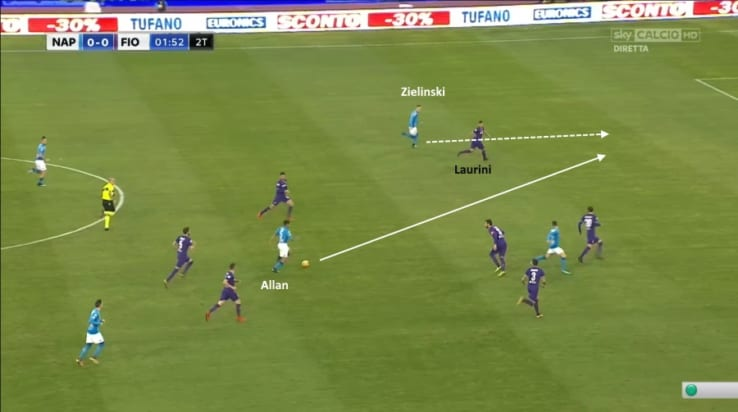
\includegraphics[scale=0.45]{filtrante2.jpg}
			\caption{Esecuzione di un passaggio filtrante} \label{fig:filt}
			Source: \url{https://www.ilmisterone.com/2019/01/16/passaggi-filtranti/}
		\end{center}
	\end{figure}
	È stata inserita per capire se un alto numero di passaggi medi possa essere determinante ai fini dell'esito della partita. 
	
	\item \textsf{MPCmp\%}: Indica la percentuale di passaggi medi riusciti ai giocatori della squadra specificata della variabile \textsf{Team}.\\ 
	È stata inserita perché permette di capire quanti passaggi siano andati a buon fine tra tutti quelli tentati e quindi ricavare la precisione dei giocatori della squadra.
	\item \textsf{LPAtt}: Indica il numero di passaggi lunghi tentati dai giocatori della squadra specificata della variabile \textsf{Team}. Per passaggi lunghi si intendono tutti quelli effettuati all'interno di una lunghezza superiore ai ventisette metri. Questi passaggi possono essere considerati come lanci lunghi per cambi di gioco o per lanciare le punte, cioè i giocatori che giocano come attaccanti, in profondità. Una rappresentazione di passaggio lungo è mostrata nella Figura \ref{fig:cambio}.\\
	\begin{figure}[ht]
		\begin{center}
			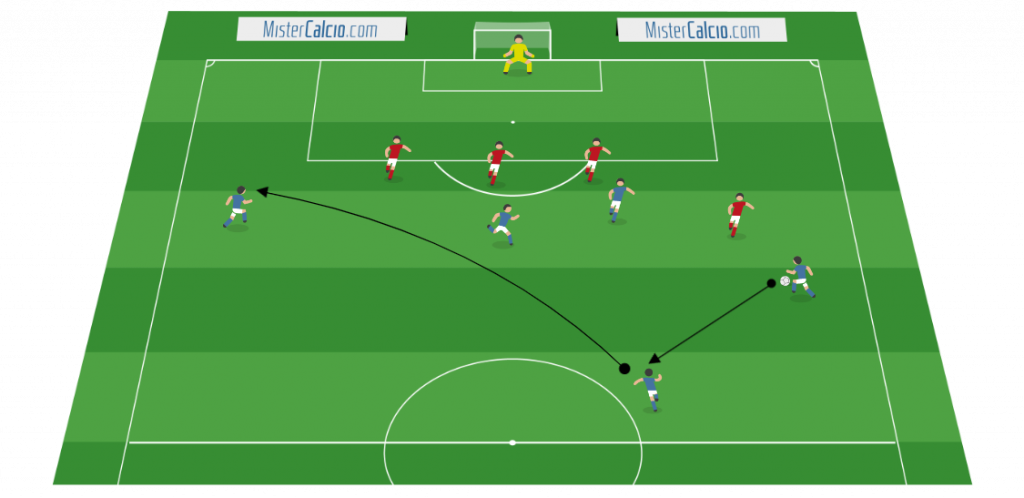
\includegraphics[scale=0.45]{cambio-di-gioco.png}
			\caption{Esecuzione di un cambio di gioco} \label{fig:cambio}
			Source: \url{https://www.mistercalcio.com/tattica/il-cambio-di-gioco/}
		\end{center}
	\end{figure}
	È stata inserita per capire se un alto numero di passaggi lunghi possa essere determinante ai fini dell'esito della partita.
	
	\item \textsf{LPCmp\%}: Indica la percentuale di passaggi lunghi riusciti ai giocatori della squadra specificata della variabile \textsf{Team}. \\
	È stata inserita perché permette di capire quanti passaggi sono andati a buon fine tra tutti quelli tentati e quindi ricavare la precisione dei giocatori della squadra.
	
	\item \textsf{Crs}: Indica il numero di cross effettuati dalla squadra specificata della variabile \textsf{Team}. Un cross (in italiano traversone) è un tipo di passaggio medio o lungo, solitamente effettuato sulle fasce laterali dell'area avversaria o comunque vicino all'area avversaria, che permette al compagno di squadra posizionato vicino alla porta avversaria di colpire la palla al volo di testa oppure di piede per segnare un possibile gol. Quindi, se eseguito correttamente, il cross può diventare un assist, cioè l'ultimo passaggio per la realizzazione del gol. 
	
	\begin{figure}[!ht]
		\begin{center}
			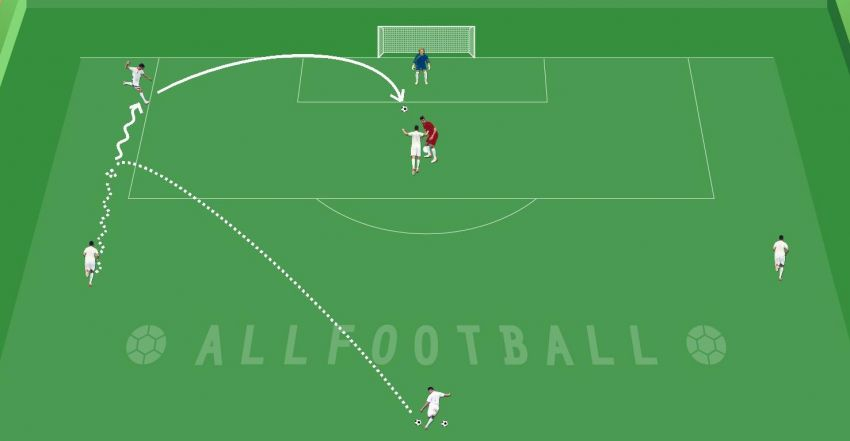
\includegraphics[scale=0.37]{cross.jpg}
			\caption{Rappresentazione di un cross} \label{fig:cross}
			Source: \url{http://www.allfootball.it/blog/calcio-vincere-allenando-i-dettagli/27-2-2017/calcio-la-marcatura-a-uomo-su-cross-laterale/}
		\end{center}
	\end{figure}
	
	Una rappresentazione di cross è mostrata nella Figura \ref{fig:cross}.
\end{itemize}

\subsection{Dati difensivi}

In questo gruppo sono contenute le variabili collegate alla fase difensiva.

\begin{itemize}
	
	\item \textsf{Saves}: Indica il numero di parate fatte del portiere della squadra specificata della variabile \textsf{Team}. \\
	È stata inserita perché permette di valutare se la squadra subisce tanti tiri dagli avversari, così come la qualità del portiere nel salvare la squadra da un possibile gol subito.
	
	\item \textsf{Int}: Indica il numero di intercettazioni fatte dai giocatori della squadra specificata della variabile \textsf{Team}. Per intercettazione della palla si intende l'intercettazione di un passaggio della squadra avversaria entrando in possesso del pallone andando ad interrompere il passaggio avversario. 
	
	\item \textsf{TklWin}: Indica il numero di contrasti vinti dai giocatori della squadra specificata della variabile \textsf{Team}. Per contrasto si intende il tentativo da parte di un giocatore difendente di sottrarre il possesso della palla all'avversario. Quindi chi ha in possesso la palla viene attaccato da chi ne è privo. Se si riesce a prendere il pallone all'avversario allora si avrà vinto il contrasto. I contrasti vengono effettuati anche per allontanare l'avversario dalle zone pericolose. La Figura \ref{fig:tackle} mostra un contrasto di gioco.\\
	\begin{figure}[!ht]
		\begin{center}
			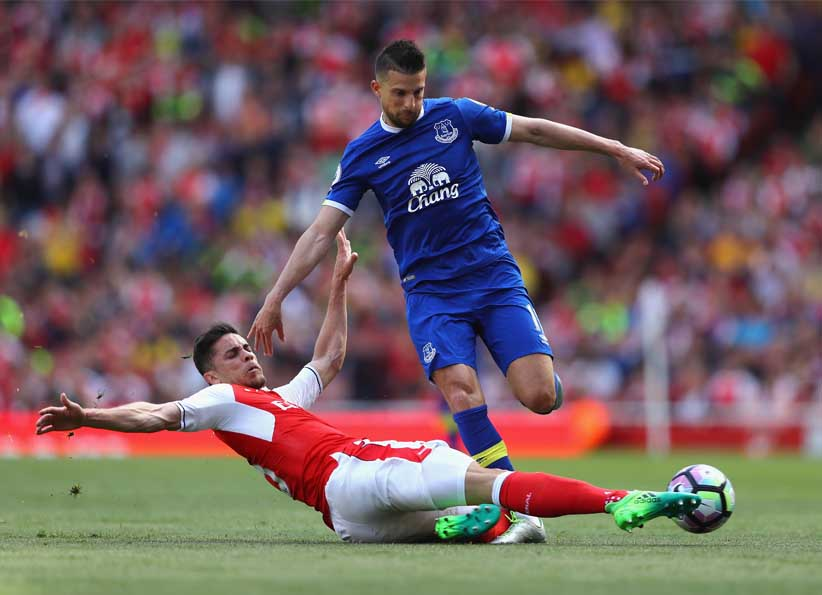
\includegraphics[scale=0.40]{tackle.jpg}
			\caption{Rappresentazione di un contrasto in scivolata}
			Source: \url{https://www.ilmisterone.com/2022/01/24/partita-solo-tackle/}
			\label{fig:tackle}
		\end{center}
	\end{figure}
	Visto che tale intervento senza palla modifica il gioco dell'avversario, si è deciso di inserire i contrasti vinti come variabile. 
	
	\item \textsf{Recov}: Indica il numero di palle vaganti recuperate dalla squadra specificata della variabile \textsf{Team}. Per palle vaganti si intendono quei palloni che, a seguito di un contrasto di gioco, non sono stati recuperati dalla squadra che ha effettuato il contrasto ma chi ha subito il contrasto, ne ha comunque perso il controllo. Quindi nessuno ha in possesso il pallone e la palla viene detta vagante.\\
	Dato che questa variabile sembra essere legata al possesso del pallone, potrebbe essere interessante per l'analisi.
	
	
\end{itemize}

Nella Tabella \ref{tab:summary} è riassunto l'insieme delle variabili presenti e le loro macro-aree di appartenenza.\\
\begin{table}[!htb]%
	
	\renewcommand{\arraystretch}{1.7}
	\centering
	\begin{tabular}{c c c c c}
		\hline	
		
		\textbf{Statistiche generali} & \textbf{Tiri} & \textbf{Possesso} & \textbf{Passaggi} & \textbf{Difensive} \\	
		\hline			
		AtHome & Sh & Poss & PAtt & Saves\\
		Res & SoT & ToDefPen & PCmp\% & Int\\
		GF & G/Sh & ToDef3rd & SPAtt & TklWin\\
		GA &  & ToMid3rd & SPCmp\% & Recov\\
		Team &  & ToAtt3rd & MPAtt&\\
		VS &  & ToAttPen & MPCmp\% &\\
		Fls &  & ToDist & LPAtt &\\
		Fld &  &  & LPCmp\% &\\
		Off &  &  & Crs \\
		\hline
		
		
	\end{tabular} \hbox{}
	
	\caption{La tabella riassuntiva delle variabili presenti nel \emph{dataset}.} \label{tab:summary}
\end{table}

Di seguito nella Tabella \ref{tab:summary2} è mostrato per ogni variabile il nome che ha all'interno del \emph{dataset}.


\begin{table}[!htb]%
	
	\renewcommand{\arraystretch}{1.7}
	\centering
	\begin{tabular}{c c }
		\hline	
		
		\textbf{Originale} & \textbf{Rinominate} \\	
		\hline			
		AtHome & AtHome \\
		Res & Res \\
		GF & GF\\
		GA & GF \\
		Team & Team \\
		VS & Vs\\
		Poss & Poss\\
		Sh & Sh\\
		SoT & SoT\\
		G/Sh & G.Sh \\
		Saves & Saves \\
		PAtt & PAtt \\
		PCmp\% & PCmp.\\
		SPAtt & SPAtt \\
		SPCmp\% & SPCmp.\\
		MPAtt & MPAtt \\
		MPCmp\% & MPCmp.\\
		LPAtt & LPAtt \\
		LPCmp\% & LPCmp. \\
		ToDefPen & ToDefPen \\
		ToDef3rd & ToDef3rd \\
		ToMid3rd & ToMid3rd \\
		ToAtt3rd & ToAtt3rd \\
		ToAttPen & ToAttPen \\
		ToDist & ToDist\\
		Fls & Fls \\
		Fld & Fld \\
		Off & Off \\
		Crs & Crs \\
		Int & Int \\
		TklWin & TklWin \\
		Recov & Recov \\
		\hline
		
	\end{tabular} \hbox{}
	
	\caption{Tabella corrispondenza tra nomi originali e nomi nel \emph{dataset}} \label{tab:summary2}
\end{table}
